\documentclass[12pt,a4paper,UTF8]{ctexart}




%设置页边距
\usepackage{geometry}
\geometry{left=2.5cm,right=2.5cm,top=2.5cm,bottom=2.5cm}
\usepackage{wrapfig}



%需要用到的扩展包
\usepackage{xeCJK,amsmath,paralist,enumerate,booktabs,multirow,graphicx,float,subfig,setspace,listings,lastpage,hyperref}
\usepackage{fancyhdr}



%设置页眉页脚以及页码
\pagestyle{fancy}
\rhead{牛顿环}
\lhead{大学基础物理实验报告}
\cfoot{Page\thepage/\pageref{LastPage}}
\rfoot{\today}




%报告中用到的图片存放在这个tex文件所在目录中的figures子目录中
\graphicspath{{figures/}}









%报告开始
\begin{document}
	
	
	
	
	%设置课程标题
	\begin{center}
		\heiti\LARGE{《大学基础物理实验》课程实验报告}
	\end{center}
	
	
	
	
	%设置实验人信息以及实验时间表格
	
	
	\begin{center}
		\begin{tabular}{lcr}
			
			{\songti 姓名及学号:2211082蒋丰毅}  \quad 专业:工科试验班 \quad 年级:22级 \quad 座号:10\\
			{\songti  学院:软件学院 \quad 实验组别:C组\quad 实验时间:2023年5月19日~星期五~上午}\\
			
			
		\end{tabular}
	\end{center}
	\vspace{-0.2cm}
	{\noindent}	 \rule[-10pt]{16cm}{0.05em}\\
	
	\vspace{-0.4cm}
	
	
	
	
	
	
	%实验题目
	\begin{center}
		\LARGE\textbf{牛顿环}
	\end{center}
	
	
	\subsection*{[实验目的]}
    \par 1.观察等厚干涉现象,并利用等厚干涉测量凸透镜表面的曲率半径。
    \par 2.了解读数显微镜的使用方法。

	\subsection*{[实验器材]}
	\par 牛顿环装置,钠灯,读数显微镜
\subsection*{[实验原理]}
\subsubsection*{牛顿环原理}
\begin{figure}[!htbp]
	\centering
	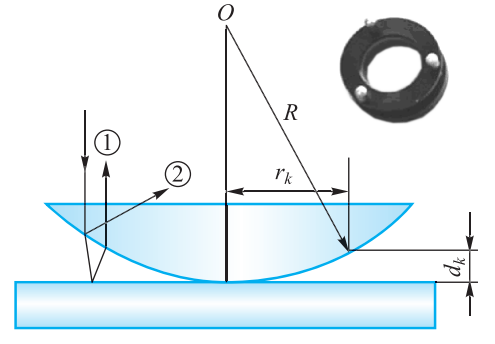
\includegraphics[width=0.5\textwidth]{牛顿环.png}
	\caption{牛顿环原理}
\end{figure}
\subsubsection*{测量原理}
\par 在图1中,在图4-1-1中,$R$为待测透镜凸面的曲率半径,$r_k$是第k级干涉环的半径,$d_k$是第k级干涉环所对应的空气间隙的厚度。如果入射光的波长为$\lambda$,则第k级干涉环所对应的光程差为
\[
	\Delta_k = 2d_k+\frac{\lambda}{2}
\]
\clearpage
\par 其中,$\dfrac{\lambda}{2}$为光由光疏介质入射到光密介质时,反射光的半波损失。因此,在接触点处($d_0$=0)的光程差为
\[
	\Delta_0 = \frac{\lambda}{2}
\]
\par 在理想情况下,牛顿环的中心是一个几何暗点。但在实际情况中,透镜和平板玻璃接触时,由于有重力和压力存在,透镜的凸面和平板玻璃均发生形变,两者的接触不再是点接触,而是面接触。因此,牛顿环的零级暗条纹不是个点,而是一个较大的暗斑。
\par 第$k$级干涉暗环处的光程差为
\[
	\Delta_k = 2d_k+\frac{\lambda}{2} = (k+\frac{1}{2})\lambda
\]
\par 所对应的空气间隙的厚度为
\[
	d_k = k\frac{\lambda}{2}
\]
\par 由于$R\gg d_k$,所以有
\[
	r_k^2 = R^2-(R-d_k)^2 \approx 2Rd_x
\]
\par 可知第$k$级别的干涉暗环的半径为
\[
	r_k = \sqrt{k\lambda R}
\]
\par 但是在实际测量中,无法确定干涉环圆心的位置,但是可以获得弦长
\[
	l_k^2 = 4(r_k^2-s^2)
\]
\par 代入之前的公式,得到
\[
	l_k^2 = 4k\lambda R-4s^2
\]
\par 为了得到斜率求出$R$,测量不同数据利用最小二乘法计算出斜率。
\subsection*{[实验内容]}
\subsubsection*{调节牛顿环装置}
\par \textbf{一、点燃钠灯}\quad 几分钟后它将发出明亮的黄光。调节半透半反镜的倾角和左右方向,使显微镜的视场达到最亮。
\par \textbf{二、找到暗纹}\quad 调节目镜,使得能够清晰的看清叉丝,将物镜的位置移动到最低,眼睛看着目镜,从下网上移动目镜,知道能够看清条纹,最后根据条纹的方向将叉丝移动到最中心的暗环处
\clearpage
\begin{figure}[!htbp]
	\centering
	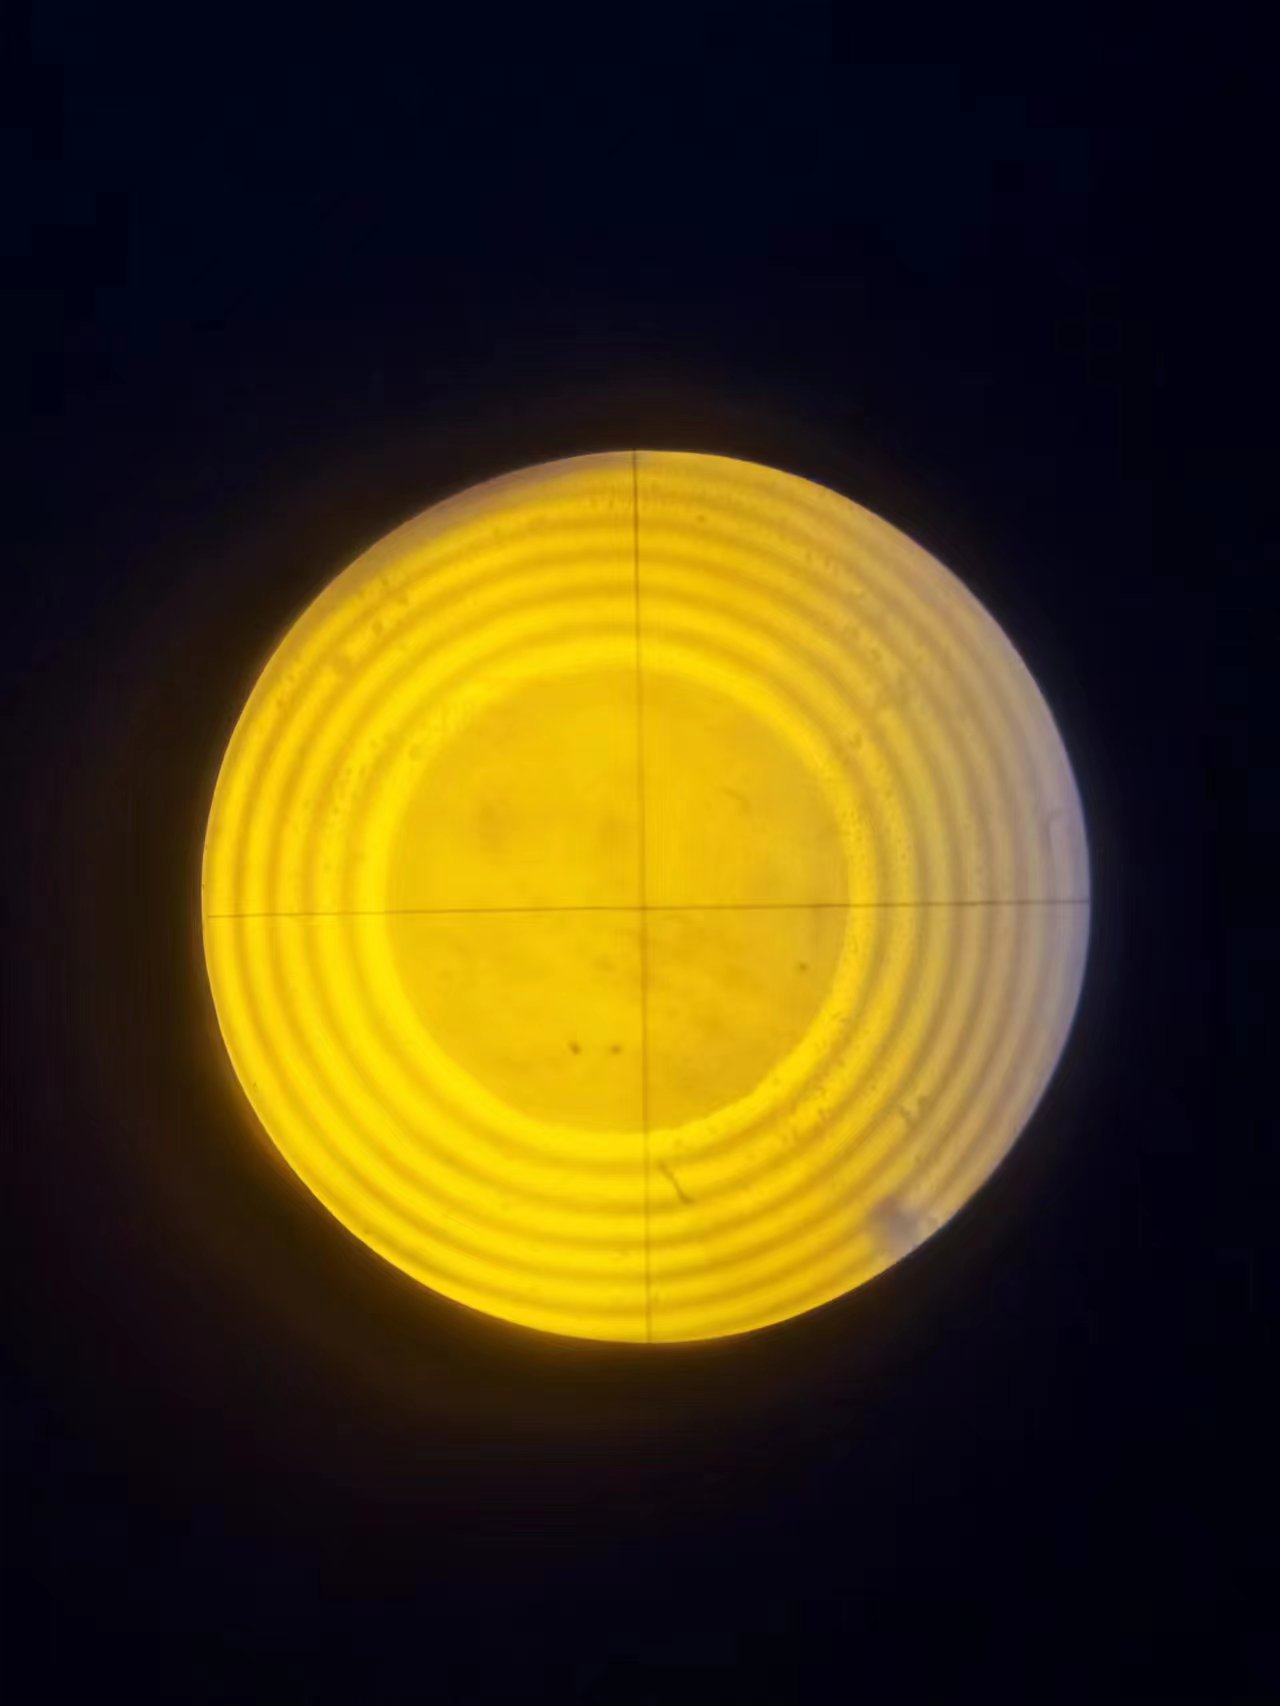
\includegraphics[width=0.5\textwidth]{牛顿环.jpg}
	\caption*{牛顿环图片}
\end{figure}

\par \textbf{三、测量}\quad 通过旋钮移动叉丝的位置,测量不同级次的干涉环的弦长,\textbf{注意:}在实验过程中,为了避免回程差,需从45级次开始,一直向同一个方向进行测量。
\subsection*{数据处理}
\par 光源波长:589.3nm

\begin{table}[!htbp]
	\centering
	\begin{tabular}{|ccc|c|c|c|c|c|c|c|}
	\hline
	\multicolumn{3}{|c|}{干涉级数}                            & 10     & 15     & 20     & 25     & 30     & 35     & 40      \\ \hline
	\multicolumn{2}{|c|}{\multirow{2}{*}{干涉位置}} & 左       & 25.679 & 26.117 & 26.527 & 26.842 & 27.139 & 27.434 & 27.744  \\ \cline{3-10} 
	\multicolumn{2}{|c|}{}                      & 右       & 19.878 & 19.395 & 18.921 & 18.559 & 18.205 & 17.901 & 17.57   \\ \hline
	\multicolumn{3}{|c|}{弦长}                              & 5.801  & 6.722  & 7.606  & 8.283  & 8.934  & 9.533  & 10.174  \\ \hline
	\multicolumn{3}{|c|}{弦长平方}                            & 33.651 & 45.185 & 57.851 & 68.608 & 79.816 & 90.878 & 103.510 \\ \hline
	\end{tabular}
	\caption{实验数据记录表(单位:$mm$)}
	\end{table}
\subsubsection*{使用最小二乘法处理数据}
\[
	l_k^2 = 4k\lambda R-4s^2
\]
\par 目的:求出直线斜率$4\lambda R$
\clearpage
\par 根据最小二乘法列出公式
$$\left\{
	\begin{aligned}
	\sum_{1=1}^{7} y_i &= 7a + b\sum_{1=1}^{7}x_i \\
	\sum_{1=1}^{7}x_iy_i & = a \sum_{1=1}^{7}x_i +b\sum_{1=1}^{7}x_i^2
	\end{aligned}
	\right.
$$
\par 解得:

$$\left\{
	\begin{aligned}
	a &= \overline{y}-b\overline{x} \\
	b & = \dfrac{\overline{xy}-\overline{x}\cdot\overline{y}}{\overline{x^2}-\overline{x}^2}
	\end{aligned}
	\right.
$$
解得$a = 2.306$,故
\[
	R^{\prime} = \frac{K}{4\lambda}=0.9785mm
\]
\subsubsection*{不确定度的计算}
\par 
\[
	\mu_{y_i} = \sqrt{\sum_{1}^{7}\frac{(y_i-a-bx_i)^2}{5}} = 0.5669
\]
\[
	S_{xx} = \sum_{1}^{7}(x_i-\overline{x})^2 = 700
\]
\[
	\mu_b = \frac{\mu_{y_i}}{\sqrt{S_{xx}}} = 0.0214
\]
则最终 $R = R^{\prime}(1\pm\mu_b) = 0.9785\pm 0.0210(mm)$
\subsection*{[思考题]}
\par 可以.
此时每一级的波程差为
\[
	\Delta_k = 2d_k = (k+1)\lambda
\]
空气间隙为
\[
	d_k = \frac{(k+1)\lambda}{2}
\]
由于$R\gg d_k$,$r_k^2 = R^2-(R-d_k)^2 \approx 2Rd_k$
$$
	r_k = \sqrt{(k+1)\lambda R}
$$
$$
	l_k^2 = 4(r_k^2-s^2)
$$
$$
	l_k^2 = ((k+1)\lambda R -s^2)
$$
\par \textbf{测量方法:}\\
与暗环类似,先找到最中央的圆,移动叉丝到第45个暗纹后,反方向转动鼓轮,每隔五个记录一次数据。\textbf{注意:}转动之后不能再改变方向!
\subsection*{考察题目}
\subsubsection*{第一题}
\par 因为不能保证叉丝移动轨迹刚好经过圆心,所以只能通过弦长的公式来计算。
\subsubsection*{第二题}
\par 先往一个方向移动超过需要测量的距离更多的距离,这样子再往回移动的过程中就可以先移动一段距离然后再测量,可以避免回空差。
\subsubsection*{第三题}
\par 1. 低级次条纹容易受到牛顿环装置接触面的灰尘、形变等影响,往往不呈比较理想的圆环形。
\par 2. 低级次条纹比较粗不利于准确测量
\par 3. 此外,由于牛顿环装置接触面的灰尘、形变等影响,低级次的条纹往往会混杂在一起,造成分辨不清,难以计数。
\subsubsection*{第四题}
\par 便于观察牛顿环现象且易于测量.如果视场过暗,则会导致无法看清干涉条纹,测量就会出现错误
\subsubsection*{第五题}
\par 1.测量时应先数45级次,然后从45级次开始测量,按级次从大到小再变大测量.测量时鼓轮必须朝一个方向转动:
\par 2.45到10级次记录暗环外圈数值,10到45级次记录内圈数值,这样就能得到相对准确的弦长值。
\end{document}
